%%%%%%%%%%%%%%%%%%%%%%%%%%%%%%%%%%%%%%%%%%%%%%%%%%%%%%%%%%%%%%%%%%%%%%%%%%%%%%%
%%                                                                           %%
%%                             Trabajo indito                               %%
%%                                                                           %%
%%%%%%%%%%%%%%%%%%%%%%%%%%%%%%%%%%%%%%%%%%%%%%%%%%%%%%%%%%%%%%%%%%%%%%%%%%%%%%%

\cabecera{cap:dop}
                 {Experiments in non-stationary problems}
\chapter{\textit{Experiments in non-stationary problems}}
\label{cap:dop}
\cabecera{cap:dop}
                 {Experiments in non-stationary problems}

%%%%%%%%%%%%%%%%%%%%%%%%%%%%%%%%%%%%%%%%%%%%%%%%%%%%%%%%%%%%%%%%%%%%%%%%%%%%%%%

%\vfill
%\itshape
%En los problemas de clasificacin de patrones se busca minimizar el nmero de patrones mal clasificados (el error), sin embargo, en muchas aplicaciones reales hay que tener en cuenta por separado el error tipo I (falsos positivos) y el error tipo II (falsos negativos).
%Suele ser un problema complejo ya que un intento de minimizar uno de ellos, hace que el otro crezca.
%Es ms, en ocasiones uno de estos tipos de error puede ser ms importante que el otro, y se debe buscar un compromiso que minimice el ms importante de los dos.
%La medida estadstica ms utilizada, significancia estadstica, es una medida del error tipo I. Sin embargo, no ofrece garantas sobre el tipo II.

%A pesar de la importancia de los errores tipo II, la mayora de los mtodos de clasificacin slo tienen en cuenta el error de clasificacin global.
%En este trabajo se propone la optimizacin de ambos tipos de error de clasificacin utilizando un algoritmo multiobjetivo en el que cada tipo de error y el tamao de red son objetivos de la funcin de evaluacin (fitness).

%Se ha utilizado una versin modificada del mtodo G-Prop (diseo y optimizacin de perceptrones multicapa usando un algoritmo evolutivo) para optimizar simultneamente la estructura de la red neuronal y los errores tipo I y II.

%Debido a la carga computacional que supone la ejecucin de un algoritmo evolutivo para el diseo de redes neuronales, se propone la paralelizacin utilizando el modelo isla como forma de distribuir la carga en una red heterognea.
%\upshape
%\clearpage

%%%%%%%%%%%%%%%%%%%%%%%%%%%%%%%%%%%%%%%%%%%%%%%%%%%%%%%%%%%%%%%%%%%%%%%%%%%%%%%
The natural evolution has shown to succeed in the changing conditions of the environments. Within any species, individuals' mating is spatially constrained, taking place between the fittest known individuals rather than just the fittest of the whole membership. This way, nature finds a way to preserve genetic diversity and responds to environmental changes (e.g. same species in different latitudes adapt to the climatic conditions). 

Within the Evolutionary Algorithms (EAs) area, spatially structured EAs (ssEA) mimic these spacial relationships in nature (see e.g. \cite{tomassini} for a survey), but they remain still unexplored in the context of non-stationary environments. Neighbourhood structures in ssEA are modeled as a graph in which the vertices are individuals and edges represent relationships between them. The impact of different neighbourhood structures on the selection pressure has been studied for regular lattices \cite{giacobini:regular} and different graph structures such as a toroid \cite{giacobini:gecco04} or small-world \cite{preuss04ppsn}.
The small-world structure has shown empirically to be competitive against panmictic EAs. Specifically in \cite{giacobini:evocop06}, a Watts-Strogatz structured population yields better results than a Barab\'asi-Albert one and standard panmictic approaches.

Nevertheless, to the extent of our knowledge, there are just two works applying ssEAs to Dynamic Optimization Problems (DOP).
 The first one, proposed by Sarma and De Jong in \cite{sarma:nsen}, explored the behaviour of a cellular Genetic Algorithm (cGA) in a non-stationary environment. More recently, Alba et al. \cite{alba:dop} did a most exhaustive investigation but then again over a cGA using a regular 2-dimensional lattice. Following this line, in this paper we analyse a small-world population applied to DOPs. Such a population structure is based on the newscast Peer-to-Peer (P2P) protocol presented in \cite{jelasity:newscast}. 

An additional advantage of using P2P protocols as population structure is that they are inherently designed to tackle large-scale graphs and they present consequently a good scalability behaviour.
In order to assess the influence of such a population structure in an EA, we have performed a scalability study on static trap functions. 
Results show that our proposal scales better than a standard GA (a generational 1-elitism GA) which has been used as a baseline for comparison. Besides, results on DOP show that our approach also outperforms the standard GA and the state of the art algorithm Self-Organizing Random Immigrants GA (SORIGA) presented in \cite{soriga}. SORIGA adopts a Self-Organized Criticality model in order to maintain a sub-population of random individuals and their offspring which varies in size by a power-law distribution.


The key to our P2P EA is the Evolvable Agent Model (EvAg) presented in \cite{laredo:cec2008}. It consists of a fine grained approach for parallelizing EAs in which there is a population of concurrent and self-scheduled agents performing the evolutionary steps of selection, variation and evaluation of individuals. Within such a study, several kinds of topologies were tested, concluding that a newscast based topology yields better results than topologies based on the Watts-Strogatz model or panmictic approaches.


The asynchronous update of the population in our approach implies a bias error during changes in DOPs (i.e. the change happens and some individuals might not be reevaluated during the first generation due to the asynchronous updating). In order to tackle with such an issue, we have assumed that the algorithm is able to detect changes. Additionally, we have also performed an exploratory study without change detections using a reduced test case in which the periods between changes are large (i.e. the larger the period is, the smaller the bias error).


\section{Results}
%%%%%%%%%%%%%%%%%%%%%%%%%%%%%%%%%%%%%%%%%%%%%%%%%%%%%%%%%%%%%
 With respect to DOPs, population size $P$ was set to 240.  In order to evaluate \emph{EvAg}'s results a standard generational GA (GGA) with 1-elitism and SORIGA were also tested with the same parameter values.

For that purpose, the DOP generator presented in \cite{yang:dop} was used to build different changing environments based on 3-trap and 4-trap functions. Given a stationary problem ($f(x)(x \in \{0,1\}^L)$) where L is the chromosome length, DOPs may be designed by applying a binary mask to each solution before its evaluation in the following manner:

\begin{equation} \label{eq:dynamic}
f(x,t)=f(x\quad XOR\quad M(k))
\end{equation}

\noindent
where t is the generation index, k = t$\tau$ is the period index and f(x, t) is the fitness of the string x. M(k) is incrementally generated as follows:

\begin{equation} \label{eq:mask}
M(k) = M(k-1)\quad XOR\quad T(k)
\end{equation}

\noindent
where $T(k)$ is an intermediate binary mask for every period k. T(k) has $\rho\times$L ones. $\rho$ is a value between 0 and 1 that controls the intensity, or severity, of changes (i.e. $\rho=0$ stands for a stationary problem and $\rho=1$ represents the highest degree of change). Therefore, by setting $\rho$ and $\tau$ it is possible to control two of the most important features of DOPs test environments: severity ($\rho$) and speed ($\tau$) of change \cite{angeline:tracking}.
 Nine different scenarios for each trap were designed by setting $\rho$ to 0.05, 0.6 and 0.95, and $\tau$ to 10, 100 and 200 generations. Stationary functions were designed with 10 subfunctions each, meaning that size of dynamic 3-trap is L = 30 and size of dynamic 4-trap is L = 40. \emph{EvAg}, GGA and SORIGA were tested with uniform crossover, bit-flip mutation, binary tournament, $p_c = 1.0$, $N = 240$ and 1-elitism (GGA). SORIGA's parameter $r_r$ was set to 3. 


GAs performance analysis on DOPs must be addressed in a different manner from static environments' usual procedure. Dynamic behaviour throughout the run must be examined, rather than the final convergence. For that purpose, the evaluation of the algorithmic performance is done by measuring the mean best-of-generation values (this is the standard procedure for DOPs). In addition, the progression of best-of-generation values may be plotted in a graph, thus helping to understand how the algorithm reacts to changes in the environment. Different mutations rates were tested, and results in table \ref{table:results} show the best configurations, that is, the mutation rates that attained the higher values when averaging the mean best-of-generation of the nine scenarios.

%%%%%%%%%%%%%%%%%%%%%%%%%%%%%%%%%%%
\begin{figure}[!htpb]
\centerline{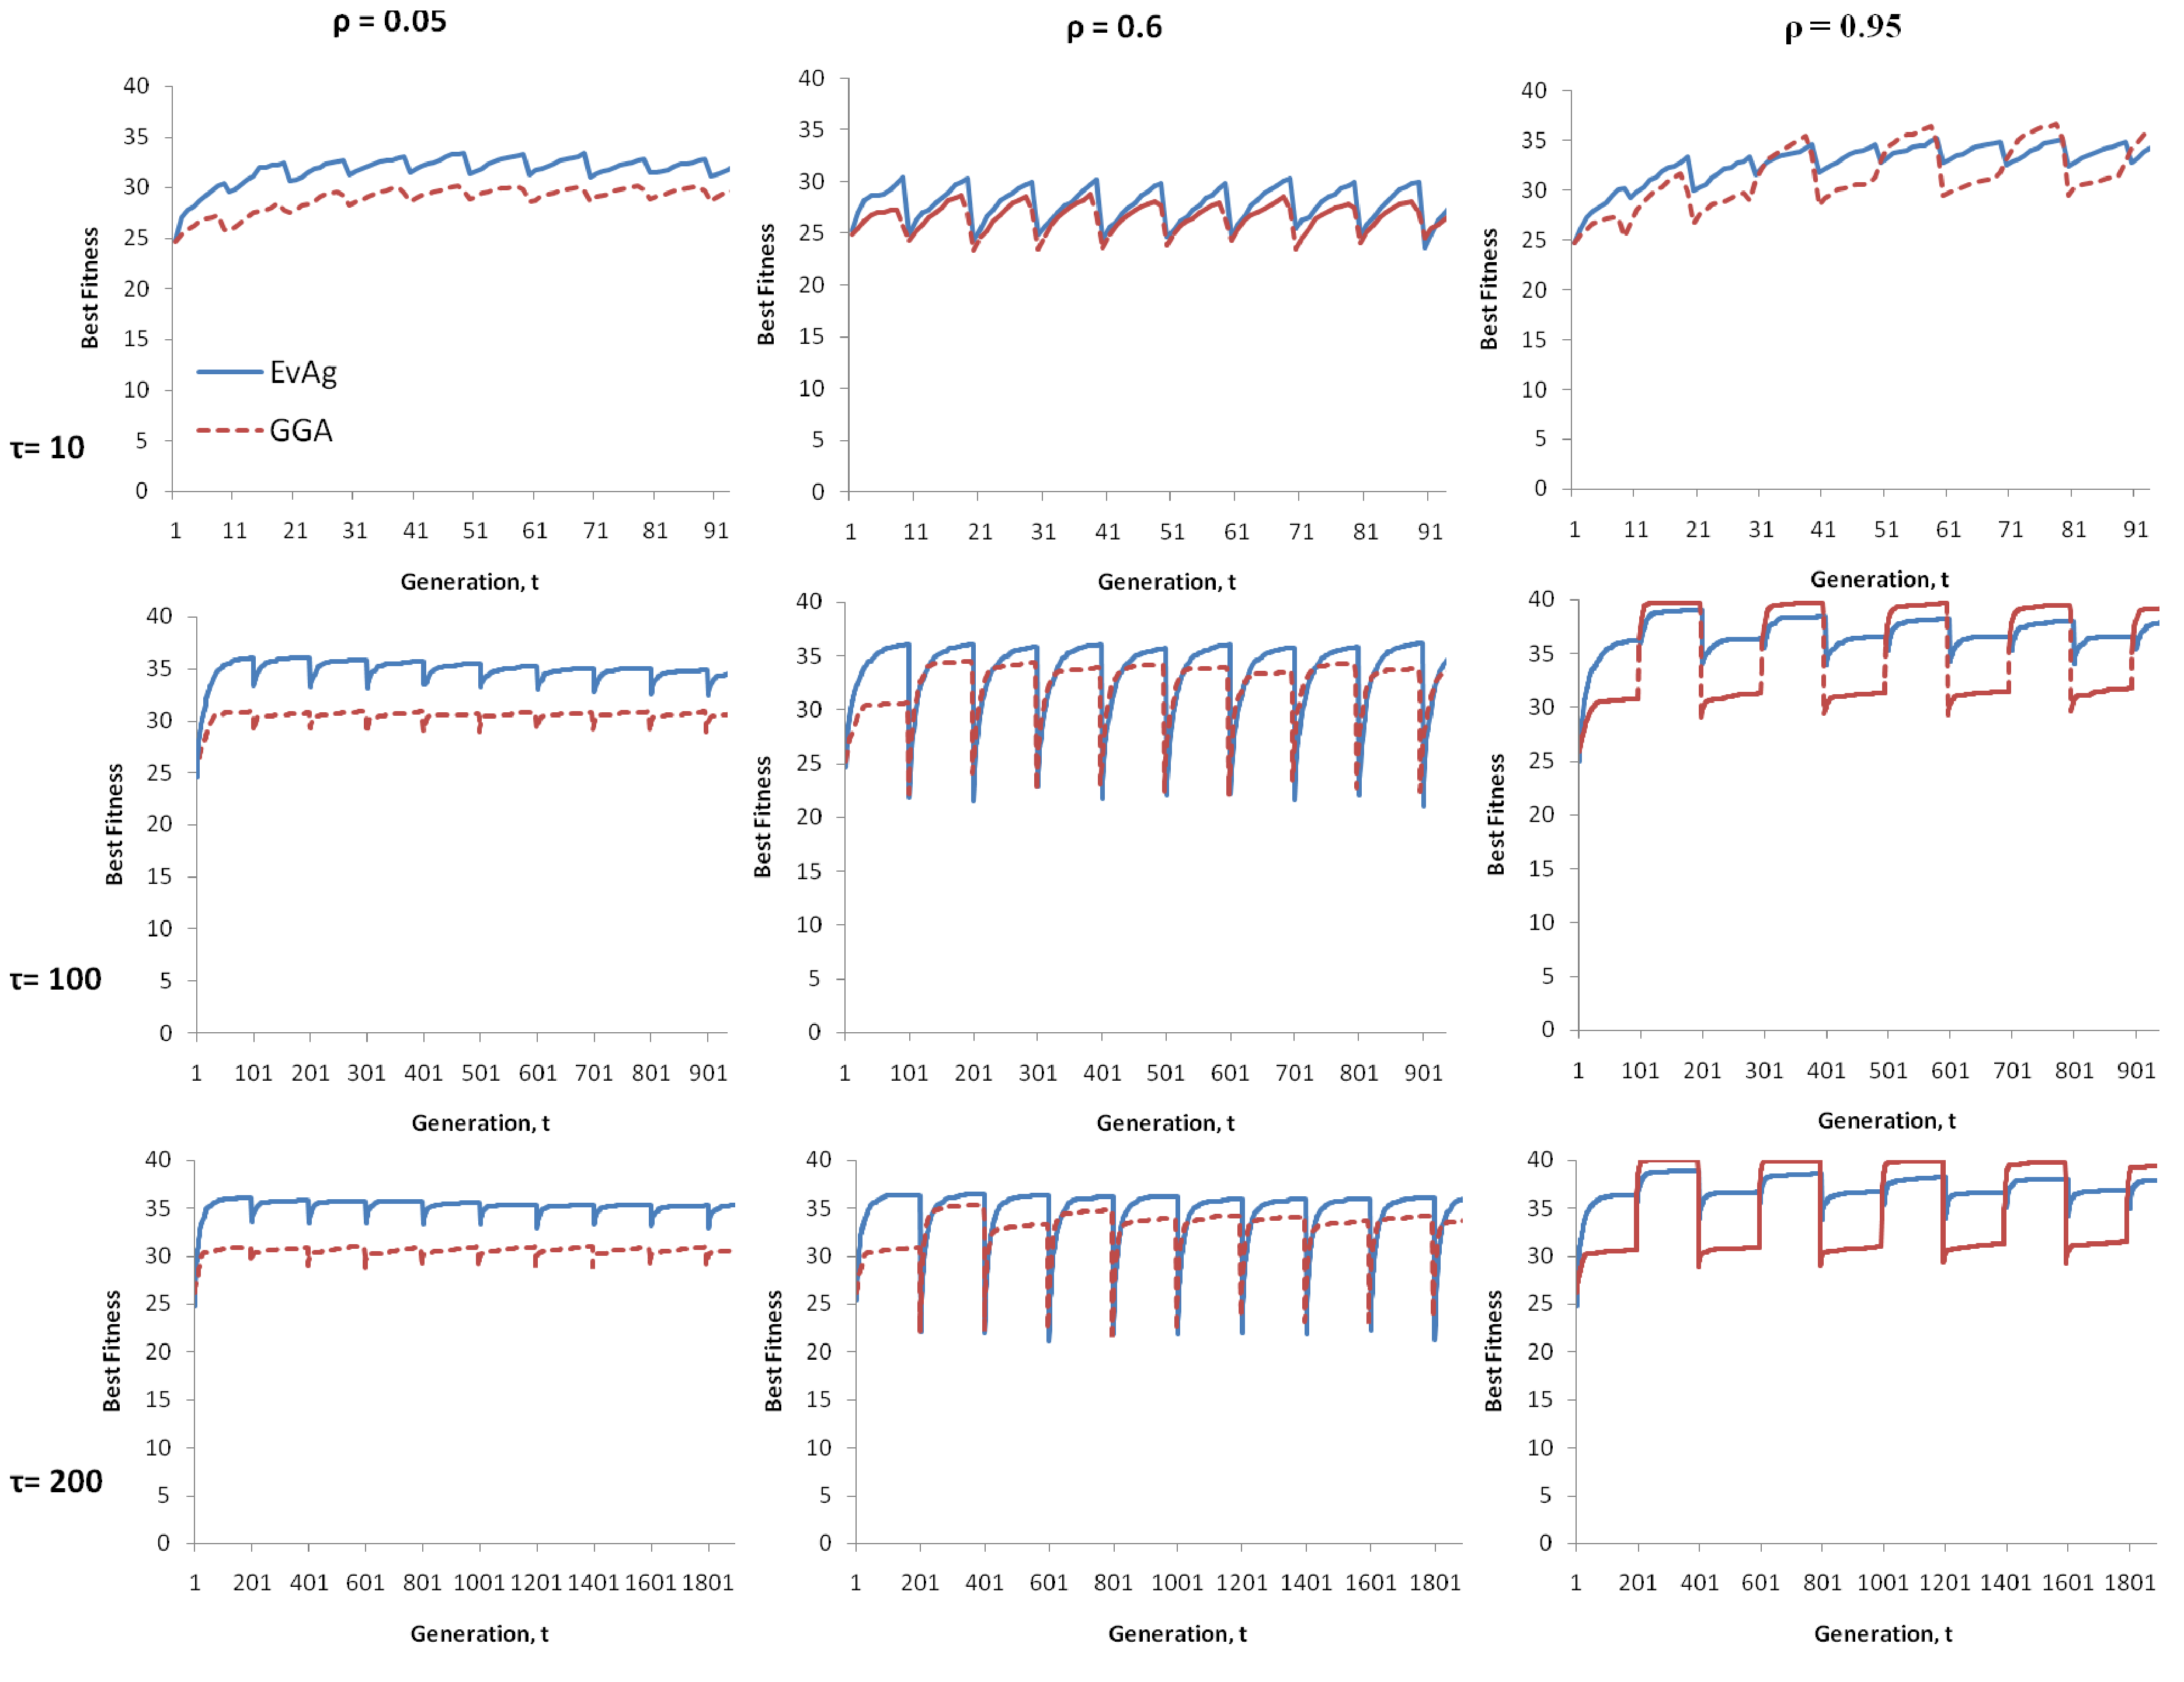
\includegraphics[width=\textwidth]{dynamic}}

\caption{Dynamics when tracking 4-trap functions ($L=40$). \textit{Best of generation} curves}
\label{fig:dynamic}
\end{figure}
%%%%%%%%%%%%%%%%%%%%%%%%%%%%%%%%%%%



%%%%%%%%%%%%%%%%%%%%%%%%%%%%%%%%%%%
\begin{table}[htbp]
\centering
{\scriptsize
\begin{tabular}{c c|c|c|c|c|c|c|c|c|c|}
\hline
&$\tau$& \multicolumn{3}{c}{10}&\multicolumn{3}{c}{100}&\multicolumn{3}{c|}{200}\\
&$\rho$&\multicolumn{1}{c}{0.05}&\multicolumn{1}{c}{0.6}&\multicolumn{1}{c}{0.95}&\multicolumn{1}{c}{0.05}&\multicolumn{1}{c}{0.6}&\multicolumn{1}{c}{0.95}&\multicolumn{1}{c}{0.05}&\multicolumn{1}{c}{0.6}&0.95\\
\hline
3-trap &GGA  &25.72&21.88&24.19& 29.4&26&25.57&29.81&26.7&25.6\\
&  $(p_m = \frac{1}{L})$ &$\pm$0.97&$\pm$0.27&$\pm$0.24& $\pm$0.44&$\pm$0.33&$\pm$0.17&$\pm$0.11&$\pm$0.33&$\pm$0.22\\
$L=30$&SORIGA & \textbf{26.43} & 22.74 & 24.10 & \textbf{29.74} & \textbf{27.71} & 26.67 & \textbf{29.86} & \textbf{28.8} & 27.95 \\
&  $(p_m = \frac{1}{2L})$& $\pm$0.62 &$\pm$0.3 &$\pm$0.26 &$\pm$0.05 & $\pm$0.17 & $\pm$0.16 &$\pm$0.02 &$\pm$0.1 &$\pm$0.16 \\
&EvAg &25.71&\textbf{22.83}&\textbf{26.37}&28.91&27.04&\textbf{27.83}&29.61&27.64&\textbf{28.03}\\
&  $(p_m = \frac{1}{L})$&$\pm$0.38&$\pm$0.43&$\pm$0.34&$\pm$0.26&$\pm$0.17&$\pm$0.39&$\pm$0.27&$\pm$0.2&$\pm$0.33\\
\hline
4-trap &GGA &28.92&26.63&31.66&30.52&32.55&35.1&30.61&33.08&35.3\\
 & $(p_m = \frac{1}{L})$&$\pm$0.33&$\pm$0.39&$\pm$0.52&$\pm$0.57&$\pm$0.34&$\pm$0.11&$\pm$0.44&$\pm$0.29&$\pm$0.129\\
$L=40$&SORIGA & 28.64 & 26.54 & 29.4 & 34.12 & 32.4 & 34.7 &\textbf{ 35.92} & 33.43 & 35.02 \\
&  $(p_m = \frac{1}{8L})$& $\pm$0.71 &$\pm$0.36 &$\pm$0.55 &$\pm$1.57 & $\pm$0.37 & $\pm$0.14 &$\pm$1.4 &$\pm$0.38 &$\pm$0.09 \\
&EvAg &\textbf{31.71}&\textbf{27.82}&\textbf{32.71}&\textbf{34.89}&\textbf{33.76}&\textbf{36.9}&35.32&\textbf{34.87}&\textbf{37.17}\\
& $(p_m = \frac{1}{L})$ &$\pm$0.53&$\pm$0.39&$\pm$0.46&$\pm$0.5&$\pm$0.28&$\pm$0.31&$\pm$0.51&$\pm$0.25&$\pm$0.33\\
\hline
\end{tabular}
}
\caption{Results on dynamic 3-trap and 4-trap (averaged over 30 independent runs). Mean of \textit{best of generation} and corresponding standard deviation values \label{table:results}}
\end{table}
%%%%%%%%%%%%%%%%%%%%%%%%%%%%%%%%%%%


%%%%%%%%%%%%%%%%%%%%%%%%%%%%%%%%%%%
\begin{table}[htbp]
\centering
{
\begin{tabular}{c c c|c|c|c|c|c|c|c|c|c|}
\hline
t-test&&$\tau$& \multicolumn{3}{c}{10}&\multicolumn{3}{c}{100}&\multicolumn{3}{c|}{200}\\
&&$\rho$&\multicolumn{1}{c}{0.05}&\multicolumn{1}{c}{0.6}&\multicolumn{1}{c}{0.95}&\multicolumn{1}{c}{0.05}&\multicolumn{1}{c}{0.6}&\multicolumn{1}{c}{0.95}&\multicolumn{1}{c}{0.05}&\multicolumn{1}{c}{0.6}&0.95\\
\hline
3-trap &EvAg vs. GGA & &$\sim$&$+$&$+$&$-$&$+$&$+$&$-$&$+$&$+$\\
&EvAg vs. SORIGA  & &$-$&$\sim$&$+$&$-$&$-$&$+$&$-$&$-$&$+$\\
\hline
 4-trap & EvAg vs. GGA &&$+$&$+$&$+$&$+$&$+$&$+$&$+$&$+$&$+$\\
& EvAg vs. SORIGA &&$+$&$+$&$+$&$+$&$+$&$+$&$+-$&$+$&$+$\\
\hline

\end{tabular}
}
\caption{Pairwise \textit{t-test} on dynamic 3-trap and 4-trap. Evolvable Agent vs. GGA and SORIGA. \label{table:ttest}}
\end{table}
%%%%%%%%%%%%%%%%%%%%%%%%%%%%%%%%%%%



Table \ref{table:ttest} helps to understand the relevance of the results in table \ref{table:results} by showing the results of pairwise t-test that compares the algorithms' performance. The ($+$) sign means that algorithm 1 is significantly better than algorithm 2, ($\sim$) means that the performance is equivalent and ($-$) means that the second GA is better. While in 3-traps GGA and SORIGA still outperform \emph{EvAg} in some scenarios, in 4-traps our proposal achieves better results, with statistical significance, in all the scenarios except one. \emph{EvAg} abilities to solve DOPs appear to emerge when facing a harder problem for GAs.




Figure \ref{fig:dynamic} shows the dynamic behaviour of \emph{EvAg} and GGA throughout the run. It is clear that \emph{EvAg} is more able to track the optimum, maintain a lower distance to the solution during the search, in all scenarios. When $\rho = 0.95$, GGA oscillates between local and global optimum, without really tracking the solution, while \emph{EvAg} maintains the best fitness closer to the global optimum, which is $f(x) = 40$.

\section{Conclusion}

In this chapter we have investigated the ability of the Evolvable Agent Model for responding to changes in dynamic optimization problems. Results show that our approach is able to outperform SORIGA \cite{soriga}, one of the state of the art algorithms in DOPs. These results are specially remarkable under deceptive conditions. The key to this is a population structure based on the small-world graph built from a P2P protocol. 

The non-generational procedure of the EvAg model produces a bias error during changes in DOPs that we have avoid by assuming that the algorithm is able to detect changes. Additionally, we have also explored its behaviour without change detections. To that end, we have used the test cases in which the periods between changes are large and the bias error is minimum. In both cases our approach outperforms the standard GA and SORIGA.

